\documentclass{article}

\usepackage[final,nonatbib]{nips_2017}

\usepackage[utf8]{inputenc} % allow utf-8 input
\usepackage[T1]{fontenc}    % use 8-bit T1 fonts
\usepackage{hyperref}       % hyperlinks
\usepackage{url}            % simple URL typesetting
\usepackage{booktabs}       % professional-quality tables
\usepackage{amsfonts}       % blackboard math symbols
\usepackage{nicefrac}       % compact symbols for 1/2, etc.
\usepackage{microtype}      % microtypography

\usepackage[backend=biber]{biblatex}
\addbibresource{report.bib}

\usepackage{graphicx}
\graphicspath{ {images/} }

% https://tex.stackexchange.com/questions/376420/include-chinese-characters-into-article-in-xelatex
\usepackage{fontspec}
\newfontfamily\cjkfont{Noto Sans CJK SC}

\title{Snowbot: An empirical study of building chatbot using seq2seq with different framework}

\author{
Pinglei Guo \\
\texttt{piguo@ucsc.edu} \\
\And
Yusi Xiang \\
\texttt{yxiang12@ucsc.edu} \\
\And
Yunzheng Zhang \\
\texttt{yzhan300@ucsc.edu} \\
\And
Weiting Zhan \\
\texttt{wzhan83@ucsc.edu} \\
}

\begin{document}

\maketitle

\begin{abstract}
    Chatbot is a growing topic, we built a open domain generative chatbot using seq2seq model with different machine learning framework (Tensorflow, MXNet).
    Our result show although seq2seq is a successful method in neural machine translation, use it solely on single turn chatbot yield pretty unsatisfactory result.
    Also existing free dialog corpus lacks both quality and quantity.
    Our conclusion is state of art technology can't build a useful open domain generative bot.
\end{abstract}

\section{Introduction}
\label{sec:introduction}

\subsection{Chatbot}
\label{subsec:chatbot}

Chatbot can be generally divided into two types, open domain and close domain.
Former can answer a wide range of questions (though the answer itself could be very general with syntax and semantic error),
latter can solve particular problems from user, and user is not expecting a close domain bot to chat freely as well.
Based on how response is generated, it can be divided to retrieval and generative,
where answer is picked from clustered responses~\cite{kannan2016smart} or generated on the fly.
In theory, open domain chatbot has more potential\footnote{if the domain is really open enough, generate random text might be the best algorithm},
and is harder to build, in practice, most chatbot that gets work done is close domain.

At first (during proposal) we believe a close domain retrieval chatbot is the most easy one in the total four combinations based on a blog post~\cite{wildml},
Then we realize that this is the most easy one in theory but the hardest one in practice, the other corner,
open domain generative is actually easiest because it's end to end, there is no need for clustering, named entity recognition, knowledge base etc.
And there is no hard metrics for evaluating a open domain chatbot~\cite{liu2016not}.
Thus we decided to build a open domain generative chatbot in the limited time given.

\subsection{Machine Learning Frameworks}
\label{subsec:ml-frameworks}

Machine learning framework is now the competing spot for tech giants, besides they are using ML excessively in their own products,
they want developers to use their framework and run it on their cloud platform, (i.e. Tensorflow on Google Cloud, MXNet on AWS, CNTK on Azure).
Although there were many open source frameworks started by individual and research organizations, most of them are deprecated
in favor of those backed by companies (i.e. Theano vs. Tensorflow)\footnote{\url{https://groups.google.com/forum/\#!msg/theano-users/7Poq8BZutbY/rNCIfvAEAwAJ}}

Tensorflow~\cite{abadi2016tensorflow} and MXNet~\cite{chen2015mxnet} are two widely used frameworks, while tensorflow is
mostly declarative, mxnet allows more imperative programming style.
A simple example is in order to debug the value of a matrix in tensorflow you need to write an op using \verb+tf.Print+ and put it inside compute graph,
while in mxnet you can just use \verb+print+ like it's a normal python variable, though in fact it might resides on GPU or other machines.
Declarative style is not very expressive, but make optimization on the framework side easier, mxnet chose to detect patterns
and only optimize critical path to gain flexibility while retain performance.
However, when it comes to most software engineers, the design and low-level API does not matter much,
community support and a wide range of up to date model is more important, and tensorflow is the obvious winner.
For researchers, mxnet might be a better choice, since it has thinner wrapper and stricter requirement.

We chose to use two higher level seq2seq frameworks, sockeye (based on mxnet)\footnote{\url{https://github.com/awslabs/sockeye}}
and OpenNMT-tf\footnote{\url{https://github.com/OpenNMT/OpenNMT-tf}} in the experiments,
we did try to write a naive one based on newer seq2seq API in tensorflow, however since both sockeye and OpenNMT-tf use state of art models
and yield unsatisfactory result, we abandoned it in the middle \footnote{\url{https://github.com/at15/snowbot/pull/23}}.

The rest of the report is organized as following, Section~\ref{sec:model} describes the basic form of the seq2seq model we are using.
Section~\ref{sec:dataset} shows how we process our dataset, and the problem in it.
Implementation detail is listed in section~\ref{sec:implementation}.
Our result is shown in section~\ref{sec:evaluation}.
Section~\ref{sec:conclusion} concludes the report.

\section{Model}
\label{sec:model}

We use seq2seq model, which is widely used in neural machine translation~\cite{sutskever2014sequence}
and can be applied to single turn dialog system (QA) as well.
Its basic structure is a recurrent neural network (RNN) and treat sentence as a sequence of words, and feed one word at each step.
The cell used in RNN is LSTM (long term short memory) to learn implicit relation ship between words
from data without explicit pre-processing.
seq2seq is one of many variants of RNN + LSTM. Based on the domain and length of input,
RNN + LSTM can be used for sequence classification, text generation, translation, dialog system etc. as shown in table~\ref{table:RNN+LSTM}

\begin{table}[h]
    \caption{Variants of RNN + LSTM}
    \label{table:RNN+LSTM}
    \centering
    \begin{tabular}{llll}
        \toprule
        Type & Input & Output & Example \\
        \midrule
        seq2one (classification) & sentence & class & Sentiment analysis \\
        seq2seq (text generation) & sentence & same sentence & Shakespeare style text \\
        seq2seq (translation) & language A & language B & NMT A -> B \\
        seq2seq (single turn QA) & question & answer & chatbot \\
        seq2seq (multi turn QA) & conversation context & answer & chatbot \\
        \bottomrule
    \end{tabular}
\end{table}

For many to many in RNN + LSTM (seq2seq), simply swap the input and output data, you get a different application for free
(Table \ref{table:seq2seq-app}).
So we can use neural machine translation framework directly to build our chatbot.

\begin{table}[h]
    \caption{Input and Output of different seq2seq application}
    \label{table:seq2seq-app}
    \centering
    \begin{tabular}{lllll}
        \toprule
        Type & Train input & Train output & Test input & Test output \\
        \midrule
        text generation & You are my foe & You are my foe & You are & my <unk>\\
        translation & {\cjkfont 你好} & Hello & {\cjkfont 你大爷} & Your uncle \\
        single turn QA & Any idea & I don't know & How's the weather & I don't know \\
        multi turn QA & Got it?; No; Why? & I don't know & Hi; Hey; What's up? & I don't know \\
        \bottomrule
    \end{tabular}
\end{table}

\begin{figure}[h]
    \centering
    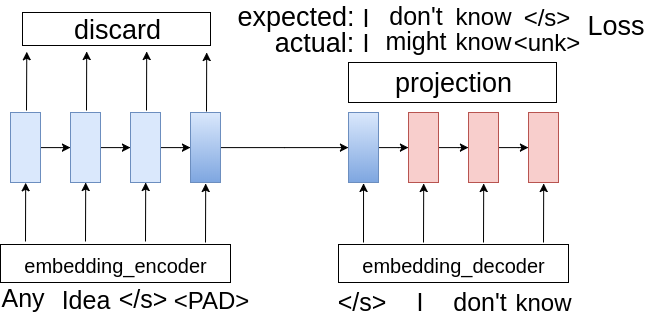
\includegraphics[width=\columnwidth]{seq2seq-simple}
    \caption{Sample figure caption.}
\end{figure}

% TODO: graph, and example text for test and train
% TODO: difference between test and train

\section{Dataset}
\label{sec:dataset}

Cornell Movie Dialog Corpus~\cite{data:cornell}

\paragraph{Paragraphs}

There is also a \verb+\paragraph+ command available, which sets the
heading in bold, flush left, and inline with the text, with the
heading followed by 1\,em of space.

\section{Implementation}
\label{sec:implementation}

\subsection{Frameworks}
\label{subsec:frameworks}

These instructions apply to everyone.

\subsection{Figures}

All artwork must be neat, clean, and legible. Lines should be dark
enough for purposes of reproduction. The figure number and caption
always appear after the figure. Place one line space before the figure
caption and one line space after the figure. The figure caption should
be lower case (except for first word and proper nouns); figures are
numbered consecutively.

You may use color figures. However, it is best for the figure
captions and the paper body to be legible if the paper is printed in
either black/white or in color.
\begin{figure}[h]
    \centering
    \fbox{\rule[-.5cm]{0cm}{4cm} \rule[-.5cm]{4cm}{0cm}}
    \caption{Sample figure caption.}
\end{figure}

\subsection{Tables}

All tables must be centered, neat, clean and legible. The table
number and title always appear before the table. See
Table~\ref{sample-table}.

Place one line space before the table title, one line space after the
table title, and one line space after the table. The table title must
be lower case (except for first word and proper nouns); tables are
numbered consecutively.

Note that publication-quality tables \emph{do not contain vertical
rules.} We strongly suggest the use of the \verb+booktabs+ package,
which allows for typesetting high-quality, professional tables:
\begin{center}
    \url{https://www.ctan.org/pkg/booktabs}
\end{center}
This package was used to typeset Table~\ref{sample-table}.

\begin{table}[t]
    \caption{Sample table title}
    \label{sample-table}
    \centering
    \begin{tabular}{lll}
        \toprule
        \multicolumn{2}{c}{Part}                   \\
        \cmidrule{1-2}
        Name & Description & Size ($\mu$m) \\
        \midrule
        Dendrite & Input terminal & $\sim$100     \\
        Axon & Output terminal & $\sim$10      \\
        Soma & Cell body & up to $10^6$  \\
        \bottomrule
    \end{tabular}
\end{table}

\section{Evaluation}
\label{sec:evaluation}
bla bla bla

\section{Conclusion}
\label{sec:conclusion}

\printbibliography

\section*{Appendix: A}
\label{sec:appendix:a}

\end{document}